\begin{frame}
  \frametitle{Strassen's Algorithm}
            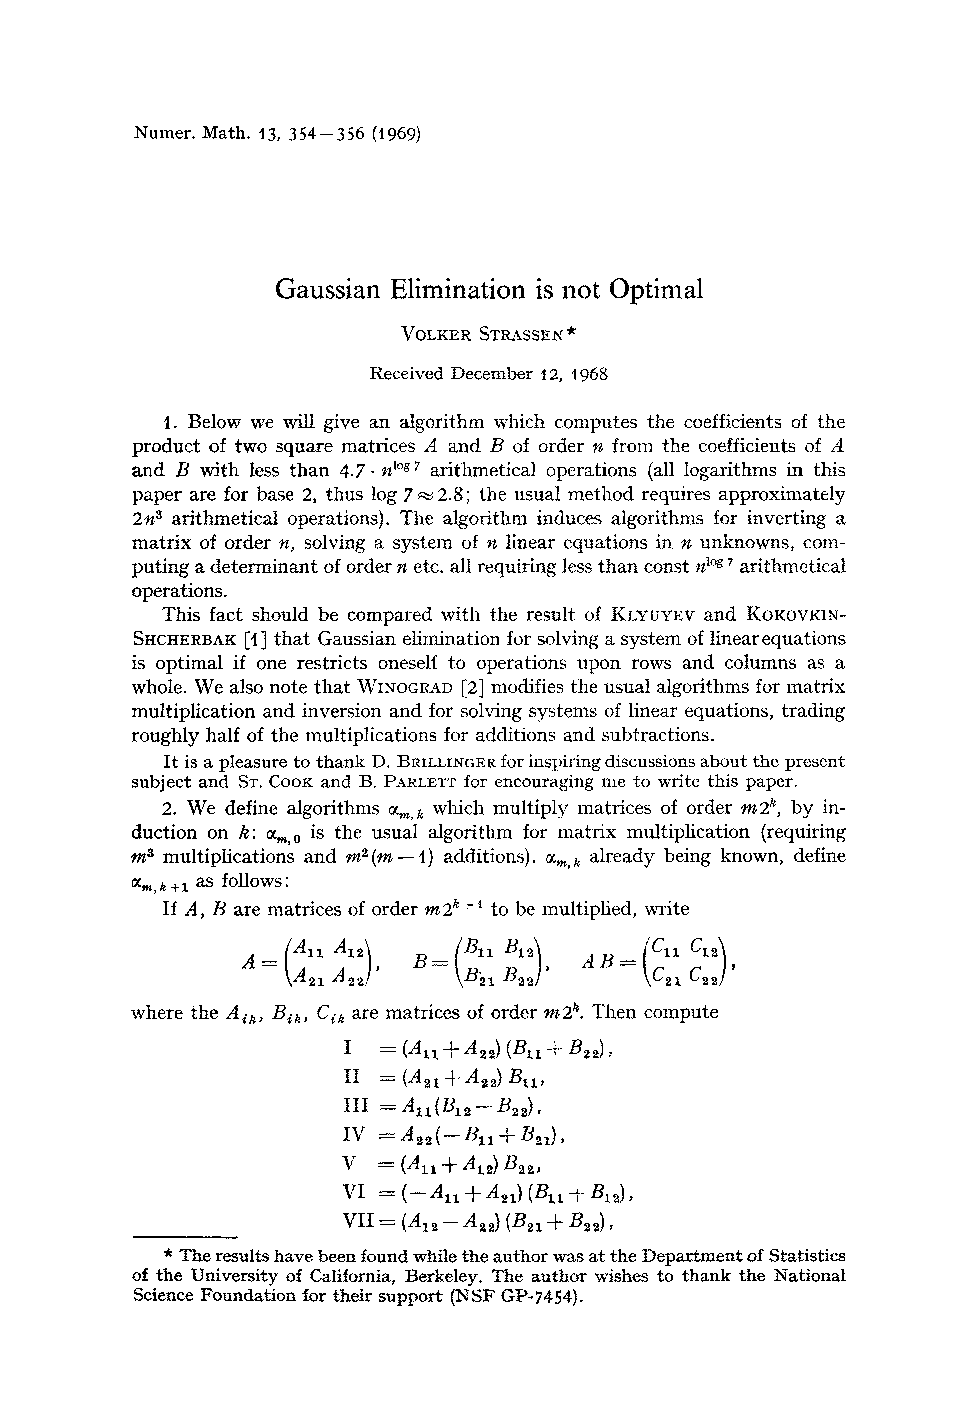
\includegraphics[page=1,width=\textwidth,height=0.8\textheight,keepaspectratio]{../papers/Strassen_original_1969.pdf}
      \includegraphics[page=2,width=\textwidth,height=0.8\textheight,keepaspectratio]{../papers/Strassen_original_1969.pdf}      \includegraphics[page=3,width=\textwidth,height=0.8\textheight,keepaspectratio]{../papers/Strassen_original_1969.pdf}
          \end{frame}

\begin{frame}
  \frametitle{Strassen's Algorithm}
  \centering
  \large
\onslide<1->{
  $
  \mathbf{A B = C}
  $
}

\onslide<2->{


\medskip
  $
  \begin{bmatrix}
  A_{11} & A_{12}\\
  A_{21} & A_{22}
  \end{bmatrix}
  \begin{bmatrix}
  B_{11} & B_{12}\\
  B_{21} & B_{22}
  \end{bmatrix}
  =
  \begin{bmatrix}
  C_{11} & C_{12}\\
  C_{21} & C_{22}
  \end{bmatrix}
  $
  }


  \onslide<3->{

\medskip
$
C_{11} = A_{11} \cdot B_{11} + A_{12} \cdot B_{21}
$

$
C_{12} = A_{11} \cdot B_{12} + A_{12} \cdot B_{22}
$

$
C_{21} = A_{21} \cdot B_{11} + A_{22} \cdot B_{21}
$

$
C_{22} = A_{21} \cdot B_{12} + A_{22} \cdot B_{22}
$
}
\end{frame}

\documentclass[border=10pt,varwidth]{standalone}
\usepackage[left=25mm,right=25mm,top=25mm,bottom=25mm]{geometry}
\usepackage[utf8]{inputenc}
\usepackage[T1]{fontenc}
\usepackage{times}
\usepackage{geometry}
\usepackage{amsmath}
\usepackage{amssymb}
\usepackage{mathrsfs}
\usepackage{amsfonts}
\usepackage{amsthm}
\usepackage{lipsum}
\usepackage{amscd}
\usepackage{graphicx}
\usepackage{fancyhdr}
\usepackage{textcomp}
\usepackage{txfonts}
\usepackage[all]{xy}
\usepackage{paralist}
\usepackage[colorlinks=true]{hyperref}
\usepackage{array}
\usepackage{tikz}
\usepackage{slashed}
\usepackage{pdfpages}
\usepackage{cite}
\usepackage{url}
\usepackage{amsmath,amsfonts,amssymb}
\usepackage{tikz}
\usetikzlibrary{arrows,matrix,positioning}
\usetikzlibrary{overlay-beamer-styles}
\usetikzlibrary{matrix.skeleton}
\usetikzlibrary{automata,positioning}
\usepackage{listings}
\usepackage{multirow}
\usepackage{color}

\begin{document}

$
A=
\begin{bmatrix}
A_{11} & A_{12}\\
A_{21} & A_{22}
\end{bmatrix},
B=
\begin{bmatrix}
B_{11} & B_{12}\\
B_{21} & B_{22}
\end{bmatrix},
C=
\begin{bmatrix}
C_{11} & C_{12}\\
C_{21} & C_{22}
\end{bmatrix}
$

\medskip
$
A \cdot B = C
$

\medskip
$
C_{11} = A_{11} \cdot B_{11} + A_{12} \cdot B_{21}\\
C_{12} = A_{11} \cdot B_{12} + A_{12} \cdot B_{22}\\
C_{21} = A_{21} \cdot B_{11} + A_{22} \cdot B_{21}\\
C_{22} = A_{21} \cdot B_{12} + A_{22} \cdot B_{22}
$

\medskip
\begin{math}
\begin{aligned}
\text{I}   &= (A_{11} + A_{22}) \cdot (B_{11} + B_{22}) \\
\text{II}  &= (A_{21} + A_{22}) \cdot B_{11} \\
\text{III} &= A_{11} \cdot (B_{12}-B_{22}) \\
\text{IV}  &= A_{22} \cdot (-B_{11}+B_{21}) \\
\text{V}   &= (A_{11} + A_{12}) \cdot B_{22} \\
\text{VI}  &= (-A_{11} + A_{21}) \cdot (B_{11} + B_{12})) \\
\text{VII} &= (A_{12} - A_{22}) \cdot (B_{21} + B_{22}) \\
\end{aligned}
\end{math}


\medskip
\begin{math}
\begin{aligned}
C_{11} &= \text{I} + \text{IV} - \text{V} + \text{VII} \\
C_{21} &= \text{II} + \text{IV} \\
C_{12} &= \text{III} + \text{V}\\
C_{22} &= \text{I} + \text{III} - \text{II} + \text{VI} \\
\end{aligned}
\end{math}


\medskip
\begin{math}
\begin{aligned}
C_{11} &= \text{II} + \text{IV} \\
C_{11} &= (A_{11} + A_{22}) \cdot (B_{11} + B_{22}) + A_{22} \cdot (-B_{11}+B_{21}) - (A_{11} + A_{12}) \cdot B_{22} + (A_{12} - A_{22}) \cdot (B_{21} + B_{22})C_{21} \\
C_{11} &= A_{11}B_{11} + A_{11}B_{22} + A_{22}B_{11} + A_{22}B_{22} -A_{22}B_{11}+A_{22}B_{21} - A_{11}B_{22} - A_{12}B_{22}+ A_{12}B_{21} + A_{12}B_{22} - A_{22}B_{21} - A_{22}B_{22} \\
C_{11} &= A_{11}B_{11} + A_{12}B_{21}
\end{aligned}
\end{math}

\section{Winograd}

$
x_1 y_1 + x_2 y_2 = (x_1 +y_2)(y_1 + x_2)-x_1 x_2 - y_1 y_2
$

$
x = (x_1, \cdots, x_n), y=(y_1, \cdots, y_n)
$

\[
\xi = \sum_{j=1}^{ \lfloor n/2 \rfloor} x_{2j-1} \cdot x_{2j}
\]

\[
\eta = \sum_{j=1}^{ \lfloor n/2 \rfloor} y_{2j-1} \cdot y_{2j}
\]

\[
\langle x,y \rangle =
\begin{cases}
 \displaystyle  \sum_{j=1}^{ \lfloor n/2 \rfloor} (x_{2j-1} + y_{2j})(x_{2j}+y_{2j-1})-\xi - \eta & \text{if  $n$ is even}\\
\displaystyle  \sum_{j=1}^{ \lfloor n/2 \rfloor} (x_{2j-1} + y_{2j})(x_{2j}+y_{2j-1})-\xi - \eta + x_n y_n & \text{if  $n$ is odd}
\end{cases}
\]

\end{document}




\begin{frame}
  \frametitle{Strassen's Algorithm}
  \begin{columns}
    \begin{column}{0.5\textwidth}
      \onslide<1->{
      \large
      \begin{math}
      \begin{aligned}
      \text{I}   &= (A_{11} + A_{22}) \cdot (B_{11} + B_{22}) \\
      \text{II}  &= (A_{21} + A_{22}) \cdot B_{11} \\
      \text{III} &= A_{11} \cdot (B_{12}-B_{22}) \\
      \text{IV}  &= A_{22} \cdot (-B_{11}+B_{21}) \\
      \text{V}   &= (A_{11} + A_{12}) \cdot B_{22} \\
      \text{VI}  &= (-A_{11} + A_{21}) \cdot (B_{11} + B_{12}) \\
      \text{VII} &= (A_{12} - A_{22}) \cdot (B_{21} + B_{22}) \\
      \end{aligned}
      \end{math}
      }
    \end{column}

    \begin{column}{0.5\textwidth}
        \onslide<2->{
        \large
        \begin{math}
        \begin{aligned}
        C_{11} &= \text{I} + \text{IV} - \text{V} + \text{VII} \\
        C_{21} &= \text{II} + \text{IV} \\
        C_{12} &= \text{III} + \text{V}\\
        C_{22} &= \text{I} + \text{III} - \text{II} + \text{VI} \\
        \end{aligned}
        \end{math}
        }
    \end{column}
\end{columns}

\onslide<3->{

\bigskip
\centering
\tiny
\begin{math}
\begin{aligned}
  C_{11} &= (A_{11} + A_{22}) \cdot (B_{11} + B_{22}) + A_{22} \cdot (-B_{11}+B_{21}) - (A_{11} + A_{12}) \cdot B_{22} + (A_{12} - A_{22}) \cdot (B_{21} + B_{22}) \\
  C_{11} &= A_{11}B_{11} + A_{11}B_{22} + A_{22}B_{11} + A_{22}B_{22} -A_{22}B_{11}+A_{22}B_{21} - A_{11}B_{22} - A_{12}B_{22}+ A_{12}B_{21} + A_{12}B_{22} - A_{22}B_{21} - A_{22}B_{22} \\
  C_{11} &= A_{11}B_{11} + A_{12}B_{21}
\end{aligned}
\end{math}
}

\end{frame}


\begin{frame}
\begin{adjustbox}{width=\textwidth}
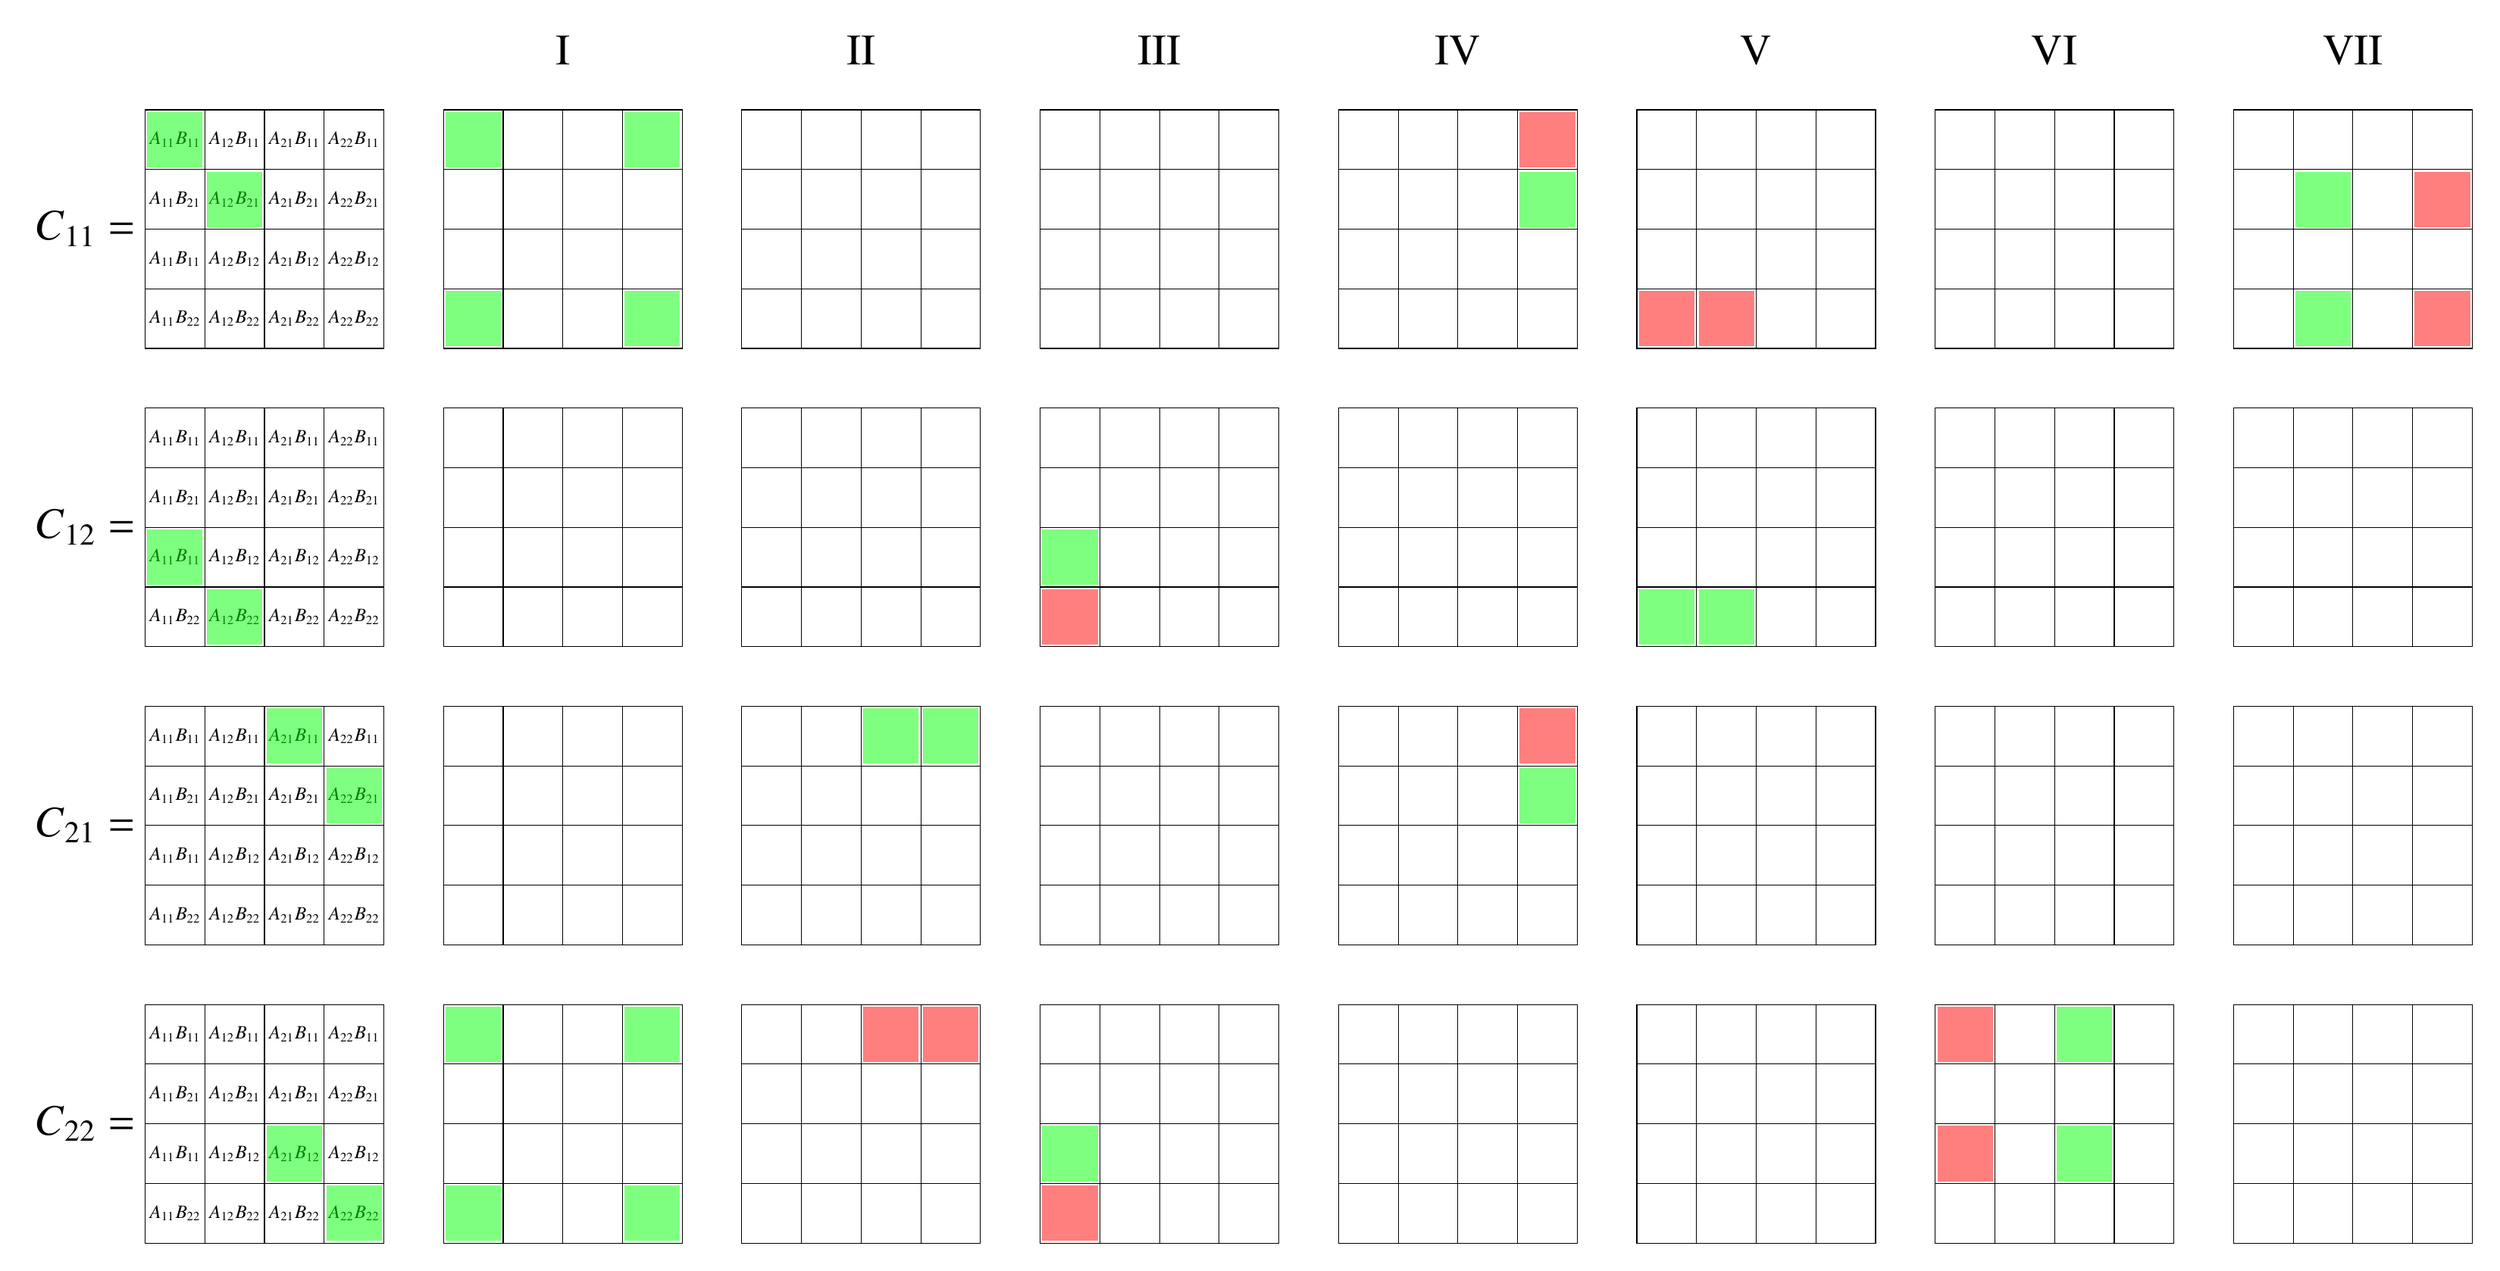
\begin{tikzpicture}[ampersand replacement=\&]

  \foreach \i in {1,...,4}
  {
  \small{
    \matrix (X\i)[matrix of math nodes,nodes in empty cells,
              nodes = {draw, minimum size=10mm,
                       anchor=center,
                       inner sep=0pt, outer sep=0pt},
              column sep=-\pgflinewidth,
              row sep=-\pgflinewidth,
              ] at (0,-\i*5)
   {
   A_{11}B_{11} \& A_{12}B_{11} \& A_{21}B_{11} \& A_{22}B_{11} \\
   A_{11}B_{21} \& A_{12}B_{21} \& A_{21}B_{21} \& A_{22}B_{21} \\
   A_{11}B_{11} \& A_{12}B_{12} \& A_{21}B_{12} \& A_{22}B_{12} \\
   A_{11}B_{22} \& A_{12}B_{22} \& A_{21}B_{22} \& A_{22}B_{22} \\
   };}

    \foreach \j in {1,...,7}
    {
    \matrix(M\i\j)[matrix of math nodes,nodes in empty cells,
                nodes = {draw, minimum size=10mm,
                         anchor=center,
                         inner sep=0pt, outer sep=0pt},
                column sep=-\pgflinewidth,
                row sep=-\pgflinewidth,
                ] at (\j*5,-\i*5)
     {
     \& \& \& \\
     \& \& \& \\
     \& \& \& \\
     \& \& \& \\
     };
   }
 }

\huge{
 \node at (-3,-20)  {$C_{22}=$};
 \node at (-3,-15) {$C_{21}=$} ;
 \node at (-3,-10) {$C_{12}=$} ;
 \node at (-3,-5) {$C_{11}=$} ;

 \node at (5,-2)  {I};
 \node at (10,-2)  {II};
 \node at (15,-2)  {III};
 \node at (20,-2)  {IV};
 \node at (25,-2)  {V};
 \node at (30,-2)  {VI};
 \node at (35,-2)  {VII};
 }


 \node[opacity=0.5, rounded corners=0pt, inner sep=-1pt, fill=green, fit=(X1-1-1)] {};
 \node[opacity=0.5, rounded corners=0pt, inner sep=-1pt, fill=green, fit=(X1-2-2)] {};
 \node[opacity=0.5, rounded corners=0pt, inner sep=-1pt, fill=green, fit=(X2-3-1)] {};
 \node[opacity=0.5, rounded corners=0pt, inner sep=-1pt, fill=green, fit=(X2-4-2)] {};
 \node[opacity=0.5, rounded corners=0pt, inner sep=-1pt, fill=green, fit=(X3-1-3)] {};
 \node[opacity=0.5, rounded corners=0pt, inner sep=-1pt, fill=green, fit=(X3-2-4)] {};
 \node[opacity=0.5, rounded corners=0pt, inner sep=-1pt, fill=green, fit=(X4-3-3)] {};
 \node[opacity=0.5, rounded corners=0pt, inner sep=-1pt, fill=green, fit=(X4-4-4)] {};

 \node[opacity=0.5, rounded corners=0pt, inner sep=-1pt, fill=green, fit=(M11-4-1)] {};
 \node[opacity=0.5, rounded corners=0pt, inner sep=-1pt, fill=green, fit=(M11-1-4)] {};
 \node[opacity=0.5, rounded corners=0pt, inner sep=-1pt, fill=green, fit=(M11-4-4)] {};
 \node[opacity=0.5, rounded corners=0pt, inner sep=-1pt, fill=green, fit=(M11-1-1)] {};
 \node[opacity=0.5, rounded corners=0pt, inner sep=-1pt, fill=red, fit=(M14-1-4)] {};
 \node[opacity=0.5, rounded corners=0pt, inner sep=-1pt, fill=green, fit=(M14-2-4)] {};
 \node[opacity=0.5, rounded corners=0pt, inner sep=-1pt, fill=red, fit=(M15-4-1)] {};
 \node[opacity=0.5, rounded corners=0pt, inner sep=-1pt, fill=red, fit=(M15-4-2)] {};
 \node[opacity=0.5, rounded corners=0pt, inner sep=-1pt, fill=red, fit=(M17-2-4)] {};
 \node[opacity=0.5, rounded corners=0pt, inner sep=-1pt, fill=red, fit=(M17-4-4)] {};
 \node[opacity=0.5, rounded corners=0pt, inner sep=-1pt, fill=green, fit=(M17-2-2)] {};
 \node[opacity=0.5, rounded corners=0pt, inner sep=-1pt, fill=green, fit=(M17-4-2)] {};

 \node[opacity=0.5, rounded corners=0pt, inner sep=-1pt, fill=green, fit=(M23-3-1)] {};
 \node[opacity=0.5, rounded corners=0pt, inner sep=-1pt, fill=red, fit=(M23-4-1)] {};
 \node[opacity=0.5, rounded corners=0pt, inner sep=-1pt, fill=green, fit=(M25-4-1)] {};
 \node[opacity=0.5, rounded corners=0pt, inner sep=-1pt, fill=green, fit=(M25-4-2)] {};

 \node[opacity=0.5, rounded corners=0pt, inner sep=-1pt, fill=green, fit=(M32-1-4)] {};
 \node[opacity=0.5, rounded corners=0pt, inner sep=-1pt, fill=green, fit=(M32-1-3)] {};
 \node[opacity=0.5, rounded corners=0pt, inner sep=-1pt, fill=red, fit=(M34-1-4)] {};
 \node[opacity=0.5, rounded corners=0pt, inner sep=-1pt, fill=green, fit=(M34-2-4)] {};

 \node[opacity=0.5, rounded corners=0pt, inner sep=-1pt, fill=green, fit=(M41-4-1)] {};
 \node[opacity=0.5, rounded corners=0pt, inner sep=-1pt, fill=green, fit=(M41-1-4)] {};
 \node[opacity=0.5, rounded corners=0pt, inner sep=-1pt, fill=green, fit=(M41-4-4)] {};
 \node[opacity=0.5, rounded corners=0pt, inner sep=-1pt, fill=green, fit=(M41-1-1)] {};
 \node[opacity=0.5, rounded corners=0pt, inner sep=-1pt, fill=red, fit=(M42-1-4)] {};
 \node[opacity=0.5, rounded corners=0pt, inner sep=-1pt, fill=red, fit=(M42-1-3)] {};
 \node[opacity=0.5, rounded corners=0pt, inner sep=-1pt, fill=green, fit=(M43-3-1)] {};
 \node[opacity=0.5, rounded corners=0pt, inner sep=-1pt, fill=red, fit=(M43-4-1)] {};
 \node[opacity=0.5, rounded corners=0pt, inner sep=-1pt, fill=green, fit=(M46-1-3)] {};
 \node[opacity=0.5, rounded corners=0pt, inner sep=-1pt, fill=red, fit=(M46-1-1)] {};
 \node[opacity=0.5, rounded corners=0pt, inner sep=-1pt, fill=green, fit=(M46-3-3)] {};
 \node[opacity=0.5, rounded corners=0pt, inner sep=-1pt, fill=red, fit=(M46-3-1)] {};
\end{tikzpicture}
\end{adjustbox}
\end{frame}


\begin{frame}
  \frametitle{Strassen's Algorithm}
  \begin{columns}
    \begin{column}{0.5\textwidth}
      \large
      \begin{math}
      \begin{aligned}
      \text{I}   &= (A_{11} + A_{22}) \cdot (B_{11} + B_{22}) \\
      \text{II}  &= (A_{21} + A_{22}) \cdot B_{11} \\
      \text{III} &= A_{11} \cdot (B_{12}-B_{22}) \\
      \text{IV}  &= A_{22} \cdot (-B_{11}+B_{21}) \\
      \text{V}   &= (A_{11} + A_{12}) \cdot B_{22} \\
      \text{VI}  &= (-A_{11} + A_{21}) \cdot (B_{11} + B_{12}) \\
      \text{VII} &= (A_{12} - A_{22}) \cdot (B_{21} + B_{22}) \\
      \end{aligned}
      \end{math}

    \end{column}

    \begin{column}{0.5\textwidth}
        \large
        \begin{math}
        \begin{aligned}
        C_{11} &= \text{I} + \text{IV} - \text{V} + \text{VII} \\
        C_{21} &= \text{II} + \text{IV} \\
        C_{12} &= \text{III} + \text{V}\\
        C_{22} &= \text{I} + \text{III} - \text{II} + \text{VI} \\
        \end{aligned}
        \end{math}

    \end{column}
\end{columns}
\end{frame}



\begin{frame}
  \frametitle{Strassen's Algorithm}

\begin{columns}
  \begin{column}{0.5\textwidth}
\large
\begin{math}
\begin{aligned}
\text{\textbf{I}}   &= (\mathbf{A_{11}} + \mathbf{A_{22}}) \cdot (\mathbf{B_{11}} + \mathbf{B_{22}}) \\
\text{\textbf{II}}  &= (\mathbf{A_{21}} + \mathbf{A_{22}}) \cdot \mathbf{B_{11}} \\
\text{\textbf{III}} &= \mathbf{A_{11}} \cdot (\mathbf{B_{12}}-\mathbf{B_{22}}) \\
\text{\textbf{IV}}  &= \mathbf{A_{22}} \cdot (-\mathbf{B_{11}}+\mathbf{B_{21}}) \\
\text{\textbf{V}}   &= (\mathbf{A_{11}} + \mathbf{A_{12}}) \cdot \mathbf{B_{22}} \\
\text{\textbf{VI}}  &= (-\mathbf{A_{11}} + \mathbf{A_{21}}) \cdot (\mathbf{B_{11}} + \mathbf{B_{12}}) \\
\text{\textbf{VII}} &= (\mathbf{A_{12}} - \mathbf{A_{22}}) \cdot (\mathbf{B_{21}} + \mathbf{B_{22}}) \\
\end{aligned}
\end{math}

\end{column}

\begin{column}{0.5\textwidth}
  \large
  \begin{math}
  \begin{aligned}
  \mathbf{C_{11}} &= \text{\textbf{I}} + \text{\textbf{IV}} - \text{\textbf{V}} + \text{\textbf{VII}} \\
  \mathbf{C_{21}} &= \text{\textbf{II}} + \text{\textbf{IV}} \\
  \mathbf{C_{12}} &= \text{\textbf{III}} + \text{\textbf{V}}\\
  \mathbf{C_{22}} &= \text{\textbf{I}} + \text{\textbf{III}} - \text{\textbf{II}} + \text{\textbf{VI}} \\
  \end{aligned}
  \end{math}

\end{column}
\end{columns}

\end{frame}

\begin{frame}
  \frametitle{Algorithm}
  \onslide<1->{

  \scalebox{0.45}{\parbox{\linewidth}{
    \begin{algorithm}[H]\caption{Strassen Matrix Multiplication}
      \setlength{\lineskip}{7pt}
      \begin{algorithmic}[1]
        \Function{strassen}{$\textbf{A}, \textbf{B}, n$}
        \If{$n = 2$}
        \State  $ \mathbf{C} \gets zeros((n, n))$
        \State $P  \gets (A[0][0]+A[1][1])\cdot( B[0][0]+B[1][1])$
        \State   $Q  \gets (A[1][0]+A[1][1])\cdot B[0][0]$
        \State   $R  \gets A[0][0]\cdot (B[0][1]-B[1][1])$
        \State   $S  \gets A[1][1]\cdot (B[1][0]-B[0][0])$
        \State   $T  \gets (A[0][0]+A[0][1])\cdot B[1][1]$
        \State   $U  \gets (A[1][0]-A[0][0])\cdot (B[0][0]+B[0][1])$
        \State   $V  \gets (A[0][1]-A[1][1])\cdot (B[1][0]+B[1][1])$
        \State   $C[0][0]  \gets P+S-T+V$
        \State   $C[0][1]  \gets R+T$
        \State   $C[1][0]  \gets Q+S$
        \State   $C[1][1]  \gets P+R-Q+U$
        \Else
      \State  $ m \gets n/2$
  \State $\mathbf{A11}, \mathbf{A12}, \mathbf{A21}, \mathbf{A22} \gets \mathbf{A}[:m][:m], \mathbf{A}[:m][m:], \mathbf{A}[m:][:m], \mathbf{A}[m:][m:]$
  \State $\mathbf{B11}, \mathbf{B12}, \mathbf{B21}, \mathbf{B22} \gets \mathbf{B}[:m][:m], \mathbf{B}[:m][m:], \mathbf{B}[m:][:m], \mathbf{B}[m:][m:]$

  \State $ \mathbf{P} \gets \text{strassen}((\mathbf{A11}+ \mathbf{A22}),(\mathbf{B11}+\mathbf{B22}), m)$
  \State $ \mathbf{Q} \gets \text{strassen}((\mathbf{A21}+ \mathbf{A22}), \mathbf{B11},m)$
  \State $ \mathbf{R} \gets \text{strassen}( \mathbf{A11},(\mathbf{B12}-  \mathbf{B22}),m)$
  \State $ \mathbf{S} \gets \text{strassen}( \mathbf{A22},(\mathbf{B21}-  \mathbf{B11}),m)$
  \State $ \mathbf{T} \gets \text{strassen}((\mathbf{A11}+ \mathbf{A12}), \mathbf{B22},m)$
  \State $ \mathbf{U} \gets \text{strassen}((\mathbf{A21}- \mathbf{A11}),(\mathbf{B11}+\mathbf{B12}),m)$
  \State $ \mathbf{V} \gets \text{strassen}((\mathbf{A12}- \mathbf{A22}),(\mathbf{B21}+\mathbf{B22}),m)$



  \State   $\mathbf{C11}  \gets \mathbf{P+S-T+V}$
  \State   $\mathbf{C12}  \gets \mathbf{R+T}$
  \State   $\mathbf{C21}  \gets \mathbf{Q+S}$
  \State   $\mathbf{C22}  \gets \mathbf{P+R-Q+U}$
  \State $  C \gets vstack((hstack((C11, C12)), hstack((C21, C22))))$

        \EndIf
        \State \textbf{return} $\textbf{C}$

       \EndFunction
      \end{algorithmic}
  \end{algorithm}
    }}}
%     \[
%   \mathcal{T}(n) = \left\{\begin{array}{lr}
%       1, & \text{if}  n \leq 2\\
%       7 \mathcal{T}(\frac{n}{2}) + n^2, & \text{if} n > 2\\
%       \end{array}\right\}
% \]
\only<2>{
    $
    \mathcal{T}(n) =
    \begin{cases}
      1  & \text{if }  n \leq 2\\
      7 \cdot \mathcal{T}(\frac{n}{2}) + n^2  & \text{if }  n > 2
    \end{cases} = \mathcal{O}(n^{\log_2 7})$

}
\only<3>{
    $
    \mathcal{T}(n) =
    \begin{cases}
      1  & \text{if }  n \leq 2\\
      7 \cdot \mathcal{T}(\frac{n}{2}) + n^2  & \text{if }  n > 2
    \end{cases} = \mathcal{O}(n^{2.81})$

}

\end{frame}

\begin{frame}
  \frametitle{Algorithm}
  \onslide<1->{

  \scalebox{0.45}{\parbox{\linewidth}{
    \begin{algorithm}[H]\caption{Strassen Matrix Multiplication}
      \setlength{\lineskip}{7pt}
      \begin{algorithmic}[1]
        \Function{MM}{$\textbf{A}, \textbf{B}, n$}
        \If{$n = 2$}
        \State  $ \mathbf{C} \gets zeros((n, n))$
                \State  $C[0, 0] \gets  A[0][0]*B[0][0]+A[0][1]*B[1][0]$
                \State  $C[0, 1] \gets  A[0][0]*B[0][1]+A[0][1]*B[1][1]$
                \State  $C[1, 0] \gets  A[1][0]*B[0][0]+A[1][1]*B[1][0]$
                \State  $C[1, 1] \gets  A[1][0]*B[0][1]+A[1][1]*B[1][1]$
        \Else
      \State  $ m \gets n/2$
  \State $\mathbf{A11}, \mathbf{A12}, \mathbf{A21}, \mathbf{A22} \gets \mathbf{A}[:m][:m], \mathbf{A}[:m][m:], \mathbf{A}[m:][:m], \mathbf{A}[m:][m:]$
  \State $\mathbf{B11}, \mathbf{B12}, \mathbf{B21}, \mathbf{B22} \gets \mathbf{B}[:m][:m], \mathbf{B}[:m][m:], \mathbf{B}[m:][:m], \mathbf{B}[m:][m:]$

    \State $\mathbf{C11} \gets \text{MM}(\mathbf{A11}, \mathbf{B11}) + \text{MM}(\mathbf{A12}, \mathbf{B21})$
    \State $\mathbf{C12} \gets \text{MM}(\mathbf{A11},\mathbf{B12}) + \text{MM}(\mathbf{A12},\mathbf{B22})$
    \State $\mathbf{C21} \gets \text{MM}(\mathbf{A21}, \mathbf{B11}) + \text{MM}(\mathbf{A22}, \mathbf{B21})$
    \State $\mathbf{C22} \gets \text{MM}(\mathbf{A21}, \mathbf{B12}) + \text{MM}(\mathbf{A22}, \mathbf{B22})$
    \State $  C \gets vstack((hstack((C11, C12)), hstack((C21, C22))))$

        \EndIf
        \State \textbf{return} $\textbf{C}$

       \EndFunction
      \end{algorithmic}
  \end{algorithm}
  \bigskip
  \bigskip
  \bigskip
  \bigskip
  \bigskip
    }}}

\only<2>{


    $
    \mathcal{T}(n) =
    \begin{cases}
      1  & \text{if }  n \leq 2\\
      8 \cdot \mathcal{T}(\frac{n}{2}) + n^2  & \text{if }  n > 2
    \end{cases} = \mathcal{O}(n^{\log_2 8})$

}
\only<3>{
    $
    \mathcal{T}(n) =
    \begin{cases}
      1  & \text{if }  n \leq 2\\
      8 \cdot \mathcal{T}(\frac{n}{2}) + n^2  & \text{if }  n > 2
    \end{cases} = \mathcal{O}(n^{3})$

}

\end{frame}
